\documentclass{scrartcl}
\usepackage{xcolor, tikz}
\usepackage{pgfplots}
\pgfplotsset{compat=newest}
\pagestyle{empty}
\definecolor{pdg2112}{RGB}{228,26,28}
\definecolor{pdg2212}{RGB}{55,126,184}
\definecolor{pdg1000010020}{RGB}{153,153,153}
\definecolor{pdg1000020040}{RGB}{166,86,40}
\definecolor{pdg11}{RGB}{152,78,163}
\definecolor{pdg1000010030}{RGB}{153,153,153}
\definecolor{pdg211}{RGB}{255,255,51}
\definecolor{pdg22}{RGB}{77,175,74}
\definecolor{pdg1000030070}{RGB}{153,153,153}
\definecolor{pdg1000050110}{RGB}{153,153,153}
\begin{document}
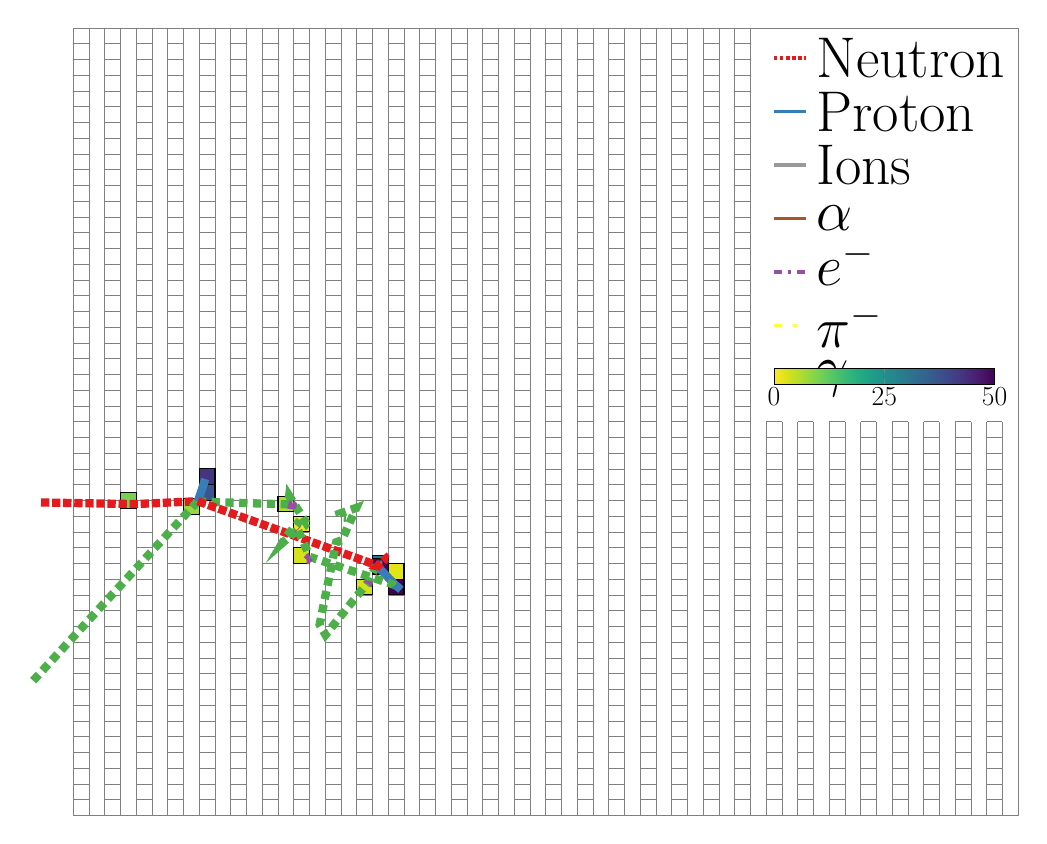
\begin{tikzpicture}[scale=0.4]
\draw[step=0.5,very thin,gray] (21.999000,-12.499) grid (22.500000,0);
\draw[step=0.5,very thin,gray] (22.999000,-12.499) grid (23.500000,0);
\draw[step=0.5,very thin,gray] (23.999000,-12.499) grid (24.500000,0);
\draw[step=0.5,very thin,gray] (24.999000,-12.499) grid (25.500000,0);
\draw[step=0.5,very thin,gray] (25.999000,-12.499) grid (26.500000,0);
\draw[step=0.5,very thin,gray] (26.999000,-12.499) grid (27.500000,0);
\draw[step=0.5,very thin,gray] (27.999000,-12.499) grid (28.500000,0);
\draw[step=0.5,very thin,gray] (28.999000,-12.499) grid (29.500000,0);
\draw[step=0.5,very thin,gray] (-0.001000,-12.499) grid (0.500000,12.499);
\draw[step=0.5,very thin,gray] (0.999000,-12.499) grid (1.500000,12.499);
\draw[step=0.5,very thin,gray] (1.999000,-12.499) grid (2.500000,12.499);
\draw[step=0.5,very thin,gray] (2.999000,-12.499) grid (3.500000,12.499);
\draw[step=0.5,very thin,gray] (3.999000,-12.499) grid (4.500000,12.499);
\draw[step=0.5,very thin,gray] (4.999000,-12.499) grid (5.500000,12.499);
\draw[step=0.5,very thin,gray] (5.999000,-12.499) grid (6.500000,12.499);
\draw[step=0.5,very thin,gray] (6.999000,-12.499) grid (7.500000,12.499);
\draw[step=0.5,very thin,gray] (7.999000,-12.499) grid (8.500000,12.499);
\draw[step=0.5,very thin,gray] (8.999000,-12.499) grid (9.500000,12.499);
\draw[step=0.5,very thin,gray] (9.999000,-12.499) grid (10.500000,12.499);
\draw[step=0.5,very thin,gray] (10.999000,-12.499) grid (11.500000,12.499);
\draw[step=0.5,very thin,gray] (11.999000,-12.499) grid (12.500000,12.499);
\draw[step=0.5,very thin,gray] (12.999000,-12.499) grid (13.500000,12.499);
\draw[step=0.5,very thin,gray] (13.999000,-12.499) grid (14.500000,12.499);
\draw[step=0.5,very thin,gray] (14.999000,-12.499) grid (15.500000,12.499);
\draw[step=0.5,very thin,gray] (15.999000,-12.499) grid (16.500000,12.499);
\draw[step=0.5,very thin,gray] (16.999000,-12.499) grid (17.500000,12.499);
\draw[step=0.5,very thin,gray] (17.999000,-12.499) grid (18.500000,12.499);
\draw[step=0.5,very thin,gray] (18.999000,-12.499) grid (19.500000,12.499);
\draw[step=0.5,very thin,gray] (19.999000,-12.499) grid (20.500000,12.499);
\draw[step=0.5,very thin,gray] (20.999000,-12.499) grid (21.500000,12.499);
\draw[very thin,gray] (0,-12.5) -- (30,-12.5) -- (30,12.5) -- (0,12.5);
\definecolor{tempcolor}{rgb}{0.458674,0.816363,0.329727}\draw[fill=tempcolor,fill opacity=1] (1.500000,-2.763140) rectangle (2.000000,-2.263140);
\definecolor{tempcolor}{rgb}{0.585678,0.846661,0.249897}\draw[fill=tempcolor,fill opacity=1] (3.500000,-2.943638) rectangle (4.000000,-2.443638);
\definecolor{tempcolor}{rgb}{0.221989,0.339161,0.548752}\draw[fill=tempcolor,fill opacity=1] (4.000000,-2.500000) rectangle (4.500000,-2.000000);
\definecolor{tempcolor}{rgb}{0.271828,0.209303,0.504434}\draw[fill=tempcolor,fill opacity=1] (4.000000,-2.000000) rectangle (4.500000,-1.500000);
\definecolor{tempcolor}{rgb}{0.688944,0.865448,0.182725}\draw[fill=tempcolor,fill opacity=1] (6.500000,-2.863160) rectangle (7.000000,-2.363160);
\definecolor{tempcolor}{rgb}{0.835270,0.886029,0.102646}\draw[fill=tempcolor,fill opacity=1] (7.000000,-4.500000) rectangle (7.500000,-4.000000);
\definecolor{tempcolor}{rgb}{0.945636,0.899815,0.112838}\draw[fill=tempcolor,fill opacity=1] (7.000000,-3.500000) rectangle (7.500000,-3.000000);
\definecolor{tempcolor}{rgb}{0.835270,0.886029,0.102646}\draw[fill=tempcolor,fill opacity=1] (9.000000,-5.500000) rectangle (9.500000,-5.000000);
\definecolor{tempcolor}{rgb}{0.160665,0.478540,0.558115}\draw[fill=tempcolor,fill opacity=1] (9.500000,-4.736453) rectangle (10.000000,-4.236453);
\definecolor{tempcolor}{rgb}{0.267004,0.004874,0.329415}\draw[fill=tempcolor,fill opacity=1] (9.500000,-4.837112) rectangle (10.000000,-4.337112);
\definecolor{tempcolor}{rgb}{0.267004,0.004874,0.329415}\draw[fill=tempcolor,fill opacity=1] (10.000000,-5.500000) rectangle (10.500000,-5.000000);
\definecolor{tempcolor}{rgb}{0.886271,0.892374,0.095374}\draw[fill=tempcolor,fill opacity=1] (10.000000,-5.000000) rectangle (10.500000,-4.500000);
\draw[color=pdg2112, line width=3pt, densely dotted] (-1.0223905832862328, -2.5659261525959614) -- (-0.02254085565728019, -2.5831471334858676) -- (0.0029999999999972713, -2.583587038178574) -- (0.48999999999998634, -2.5919749163382972) -- (0.9899999999999863, -2.6005867008965344) -- (1.4899999999999864, -2.6091984854547716) -- (1.9701691931358254, -2.617468712740349) -- (1.990000000000009, -2.6165552085227706) -- (2.4899999999999864, -2.593522756443652) -- (2.9899999999999864, -2.5704903043645313) -- (3.4899999999999864, -2.5474578522854108) -- (3.953109522650652, -2.5261247565097396);
\draw[color=pdg1000050110, line width=3pt, solid] (3.953109522650652, -2.5261247565097396);
\draw[color=pdg22, line width=3pt, dotted] (3.953109522650652, -2.5261247565097396) -- (3.5100000000000136, -3.0094085457933217) -- (3.069359004821604, -3.4899999999999998) -- (3.009999999999991, -3.554740754400123) -- (2.766356922495561, -3.8204735895346245) -- (2.745511876650653, -3.843208539312837) -- (2.7276446944978714, -3.862695639122733) -- (2.712755376037239, -3.878934888964314) -- (2.5100000000000136, -4.100072963006873) -- (2.1524866981639663, -4.49) -- (2.0100000000000136, -4.645405171613659) -- (1.5100000000000136, -5.190737380220476) -- (1.2356143915063513, -5.49) -- (1.009999999999991, -5.736069588827268) -- (0.5100000000000137, -6.28140179743406) -- (0.3187420848487591, -6.49) -- (0.010000000000013642, -6.826734006040856) -- (-0.6560484485415372, -7.55316934900547) -- (-1.3150968970830945, -8.271970041049592);
\draw[color=pdg22, line width=3pt, dotted] (3.953109522650652, -2.5261247565097396) -- (3.990000000000009, -2.5310616537131607) -- (4.056506965627795, -2.5399620008002053) -- (4.490000000000009, -2.5536183851719914) -- (4.526085150060885, -2.5547551800920267) -- (4.539591951140915, -2.5551806865074855) -- (4.573358953840989, -2.556244452546133) -- (4.613879357081077, -2.5575209717925094) -- (4.6476463597811515, -2.558584737831157) -- (4.661153160861159, -2.5590102442466156) -- (4.990000000000009, -2.569369946660821) -- (5.489999999999986, -2.58512150814965) -- (5.989999999999986, -2.6008730696384794) -- (6.489999999999986, -2.6166246311273094) -- (6.828001295278682, -2.627272727499082) -- (6.85418700890641, -2.3833482578352467) -- (6.8567353155202, -2.3596103392070975) -- (6.866080405761363, -2.3743890111559134) -- (6.8769038661501325, -2.3915056324307296) -- (6.989999999999986, -2.570360048783535) -- (6.99699999999998, -2.58143010813792) -- (7.0029999999999974, -2.5909187304417065) -- (7.007999999999993, -2.598825915694839) -- (7.255353559947321, -2.99) -- (7.4071499600774136, -3.2300564513175787) -- (7.4271442493993165, -3.2072711629903212);
\draw[color=pdg11, line width=3pt, dashdotted] (7.4271442493993165, -3.2072711629903212);
\draw[color=pdg11, line width=3pt, dashdotted] (7.4071499600774136, -3.2300564513175787);
\draw[color=pdg11, line width=3pt, dashdotted] (6.8567353155202, -2.3596103392070975);
\draw[color=pdg11, line width=3pt, dashdotted] (6.828001295278682, -2.627272727499082) -- (6.8979582291707855, -2.6468240076764658) -- (6.941960329459812, -2.650851513082467) -- (6.959567662146219, -2.646981165787932) -- (6.9621609236955235, -2.6368262969972927) -- (6.955196924235883, -2.629423160346391) -- (6.949279959396426, -2.6265917056869625);
\draw[color=pdg11, line width=3pt, dashdotted] (4.056506965627795, -2.5399620008002053);
\draw[color=pdg2212, line width=3pt, solid] (3.953109522650652, -2.5261247565097396) -- (3.990000000000009, -2.426550415674909) -- (3.9970000000000026, -2.4066139720688398) -- (4.002999999999974, -2.389657734889464) -- (4.007999999999993, -2.3755275372399103) -- (4.049868513390811, -2.255056998837148) -- (4.0800505713052875, -2.1614867057209324) -- (4.104669825435667, -2.086750825497348) -- (4.124302889420619, -2.0277731694893313) -- (4.130137017415109, -2.0100000000000002) -- (4.150097245797724, -1.9494818930907094) -- (4.159433324886391, -1.9169681446012459) -- (4.1671288086577984, -1.8911969022676485) -- (4.173351270368949, -1.870681652102966) -- (4.178405110133963, -1.8536745231400222) -- (4.182464110612796, -1.8403148629032908) -- (4.18567554297565, -1.829565570992593) -- (4.188254822451654, -1.8211415908731496);
\draw[color=pdg2112, line width=3pt, densely dotted] (3.953109522650652, -2.5261247565097396) -- (3.990000000000009, -2.5393208850095887) -- (4.489999999999986, -2.718176370869565) -- (4.989999999999986, -2.8970318567295488) -- (5.249897376989679, -2.99) -- (5.269466248378626, -2.9969999999999994) -- (5.286239566711993, -3.0029999999999997) -- (5.300217331989825, -3.008) -- (5.490000000000009, -3.075887342589531) -- (5.989999999999986, -3.254742828449507) -- (6.489999999999986, -3.433598314309491) -- (6.989999999999986, -3.6124538001694746) -- (7.489999999999986, -3.7913092860294584) -- (7.989999999999986, -3.970164771889442) -- (8.045450432552252, -3.9899999999999998) -- (8.065019303941199, -3.997) -- (8.081792622274588, -4.003) -- (8.095770387552397, -4.008000000000001) -- (8.489999999999986, -4.149020257749416) -- (8.989999999999986, -4.3278757436093995) -- (9.443226960333527, -4.49) -- (9.462795831722474, -4.497) -- (9.479569150055863, -4.503) -- (9.497000000000003, -4.509235206271421) -- (9.628509852279512, -4.556277723321076);
\draw[color=pdg1000050110, line width=3pt, solid] (9.628509852279512, -4.556277723321076);
\draw[color=pdg22, line width=3pt, dotted] (9.628509852279512, -4.556277723321076) -- (9.61207788667939, -4.591098404386349) -- (9.60273060295251, -4.610906064248889) -- (9.594718645472335, -4.6278840584167815) -- (9.588042014238862, -4.642032386890024) -- (9.510000000000014, -4.807409807561139) -- (9.50300000000002, -4.822243380938095) -- (9.497000000000003, -4.834957872404095) -- (9.492000000000008, -4.845553281959063) -- (9.423835236150376, -4.99) -- (9.393512332430713, -5.054256716761168) -- (9.042238447506588, -5.49) -- (9.009999999999991, -5.529990695482769) -- (8.509999999999991, -6.150223656058451) -- (8.236089739227827, -6.49) -- (8.010000000000014, -6.7704566166341165) -- (7.8221399093255055, -6.445661296753913) -- (7.990000000000009, -5.612149746050088) -- (7.992000000000007, -5.602218718998347) -- (7.99699999999998, -5.577391151368883) -- (8.002999999999997, -5.547598070213377) -- (8.007999999999992, -5.522770502583862) -- (8.010000000000014, -5.512839475532041) -- (8.11126635903995, -5.01) -- (8.211960878829586, -4.51) -- (8.312655398619222, -4.01) -- (8.349122755489248, -3.8289208462077156) -- (8.490000000000009, -3.7788429349938752) -- (8.52967805950625, -3.7647384971338704) -- (8.862887219235176, -3.0137713097299637) -- (8.875998094082002, -2.9842227918677127) -- (8.887235986807832, -2.9588954908429246) -- (8.896600897412714, -2.937789406655601) -- (8.98562536896361, -2.7371512937505447) -- (8.961310376554342, -2.7456302627846467) -- (8.694293824018223, -2.8387425715380497) -- (8.509999999999991, -2.9030083381369627) -- (8.502999999999975, -2.9054493334800737) -- (8.497000000000003, -2.9075416152027334) -- (8.491999999999985, -2.909285183304959) -- (8.452159145903511, -2.9231782317785315) -- (8.470362509644838, -2.99) -- (8.472269426351478, -2.997) -- (8.473903926385741, -3.003) -- (8.475266009747633, -3.008) -- (8.484121913268382, -3.040508669324233) -- (8.657005267917839, -3.0500020618646078);
\draw[color=pdg11, line width=3pt, dashdotted] (8.657005267917839, -3.0500020618646078);
\draw[color=pdg11, line width=3pt, dashdotted] (8.484121913268382, -3.040508669324233);
\draw[color=pdg11, line width=3pt, dashdotted] (8.452159145903511, -2.9231782317785315);
\draw[color=pdg11, line width=3pt, dashdotted] (8.98562536896361, -2.7371512937505447);
\draw[color=pdg11, line width=3pt, dashdotted] (8.52967805950625, -3.7647384971338704);
\draw[color=pdg11, line width=3pt, dashdotted] (8.349122755489248, -3.8289208462077156);
\draw[color=pdg11, line width=3pt, dashdotted] (7.8221399093255055, -6.445661296753913);
\draw[color=pdg11, line width=3pt, dashdotted] (7.9918722006689675, -6.792943533929721);
\draw[color=pdg11, line width=3pt, dashdotted] (9.393512332430713, -5.054256716761168) -- (9.384007396140078, -5.092042956371378) -- (9.376110593719023, -5.1274035952710175) -- (9.36997852697159, -5.1529910383841235) -- (9.36807247535803, -5.154359056417388);
\draw[color=pdg2212, line width=3pt, solid] (9.628509852279512, -4.556277723321076) -- (9.645323106344927, -4.5541588998538) -- (9.663794401991344, -4.5519492907896595) -- (9.70995534023839, -4.547014414981025) -- (9.738914739349525, -4.544306462126338) -- (9.762519124926257, -4.54232681327704) -- (9.78144758720714, -4.540802698975606) -- (9.796498695058608, -4.5399026474208055) -- (9.808311007486896, -4.539000744727999) -- (9.817899589761009, -4.538263824592727);
\draw[color=pdg2212, line width=3pt, solid] (9.628509852279512, -4.556277723321076) -- (9.90199035982955, -4.847596740189452) -- (9.990000000000009, -4.940671826772794) -- (10.036905283560282, -4.99) -- (10.23446618157459, -5.196153024734002);
\draw[color=pdg1000050110, line width=3pt, solid] (10.23446618157459, -5.196153024734002);
\draw[color=pdg22, line width=3pt, dotted] (10.23446618157459, -5.196153024734002) -- (10.010000000000014, -5.121862212778974) -- (10.002999999999975, -5.119545446484652) -- (9.997000000000003, -5.117559646803818) -- (9.991999999999985, -5.115904813736447) -- (9.879856444805863, -5.078789041050989) -- (9.608126387525408, -4.988855464213971) -- (9.509999999999991, -4.956378906042308) -- (9.502999999999975, -4.954062139747993) -- (9.497000000000003, -4.952076340067158) -- (9.491999999999985, -4.9504215069997874) -- (9.009999999999991, -4.790895599305654) -- (9.002999999999975, -4.788578833011339) -- (8.997000000000003, -4.7865930333305045) -- (8.991999999999985, -4.784938200263133) -- (8.792936215684108, -4.719054733702921) -- (8.521206158403675, -4.629121156865905) -- (8.502999999999975, -4.623095526274679) -- (8.497000000000003, -4.621109726593844) -- (8.491999999999985, -4.619454893526473) -- (8.161287205806639, -4.51) -- (8.155244300212598, -4.508000000000001) -- (8.140137036227475, -4.503) -- (8.122008319445332, -4.497) -- (8.106901055460208, -4.491999999999999) -- (8.100858149866166, -4.49) -- (8.009999999999991, -4.459928985832341) -- (8.002999999999975, -4.457612219538026) -- (7.9970000000000026, -4.455626419857191) -- (7.991999999999985, -4.453971586789821) -- (7.977746043842762, -4.449254003191871) -- (7.7060159865623294, -4.359320426354854) -- (7.5156898335709, -4.296328824043876) -- (7.509999999999991, -4.28353321692026) -- (7.50300000000002, -4.267791236289588) -- (7.497000000000026, -4.254298110034633) -- (7.492000000000007, -4.243053838155488) -- (7.388367750326052, -4.01) -- (7.166032322396314, -3.5099999999999993) -- (7.130447949521681, -3.4299759273500476) -- (7.163494135644669, -3.3942704422076444) -- (7.053798421321335, -3.4899999999999998) -- (7.010000000000014, -3.5282221268256264) -- (6.640522103106832, -3.850659114467411) -- (6.767669566963287, -3.6358012306540326) -- (6.990000000000009, -3.3820148633973184) -- (7.0029999999999974, -3.3671755868787074) -- (7.1987944936056465, -3.1436795383065417);
\draw[color=pdg11, line width=3pt, dashdotted] (7.1987944936056465, -3.1436795383065417);
\draw[color=pdg11, line width=3pt, dashdotted] (6.767669566963287, -3.6358012306540326);
\draw[color=pdg11, line width=3pt, dashdotted] (6.640522103106832, -3.850659114467411);
\draw[color=pdg11, line width=3pt, dashdotted] (7.163494135644669, -3.3942704422076444);
\draw[color=pdg11, line width=3pt, dashdotted] (7.130447949521681, -3.4299759273500476) -- (7.115277299611785, -3.4139045850684417);
\draw[color=pdg11, line width=3pt, dashdotted] (7.5156898335709, -4.296328824043876) -- (7.509999999999991, -4.2974419625487705) -- (7.497000000000026, -4.302977839441993) -- (7.492000000000007, -4.305722594577352) -- (7.468983681853478, -4.342883365312936) -- (7.443389452692463, -4.36602235486694) -- (7.425114814457265, -4.390618872625725) -- (7.405748782484716, -4.39204775197549);
\draw[color=pdg2212, line width=3pt, solid] (10.23446618157459, -5.196153024734002) -- (10.27344287996841, -5.226406102756152) -- (10.304127078223383, -5.251010508963387) -- (10.328619259849825, -5.271398207330942) -- (10.348440726694616, -5.288073485272813) -- (10.365567526872336, -5.301858779515036) -- (10.379135318036242, -5.312985491474449) -- (10.39001556163721, -5.321755050847142) -- (10.398356696947484, -5.328942039588296) -- (10.404957886019996, -5.334677649906924);
\draw[color=pdg2212, line width=3pt, solid] (10.23446618157459, -5.196153024734002) -- (10.24576683636676, -5.217516602374466) -- (10.254401566430897, -5.234486700519647) -- (10.261082263808953, -5.248161993003438) -- (10.265982990663247, -5.259250499802079) -- (10.270178576627496, -5.268122773218618) -- (10.273290933406155, -5.275364369871811);
\draw[color=pdg211, line width=3pt, loosely dashdotted] (9.628509852279512, -4.556277723321076) -- (9.680775228139987, -4.57746156629147) -- (9.710982749442474, -4.589842764114221) -- (9.736119932637848, -4.600293457484063) -- (9.75706758530066, -4.609002368625599);
\draw[color=pdg1000030070, line width=3pt, solid] (9.7640562126634, -4.611914534795217);
\draw[color=pdg2112, line width=3pt, densely dotted] (9.7640562126634, -4.611914534795217) -- (9.668442607513702, -4.592793497273311) -- (9.65868286262039, -4.590841720138484) -- (9.935383775606965, -4.344202410023877) -- (9.941407390759991, -4.351845939942709) -- (9.989999999999986, -4.3630340097651885) -- (10.002999999999997, -4.366027158516966);
\draw[color=pdg2212, line width=3pt, solid] (9.9384459618841, -4.341472908690887);
\draw[color=pdg2212, line width=3pt, solid] (9.65868286262039, -4.590841720138484);
\draw[color=pdg1000010030, line width=3pt, solid] (9.7640562126634, -4.611914534795217);
\draw[color=pdg1000020040, line width=3pt, solid] (9.7640562126634, -4.611914534795217);
\draw[color=pdg1000010020, line width=3pt, solid] (9.7640562126634, -4.611914534795217);
\draw[color=pdg1000010020, line width=3pt, solid] (9.7640562126634, -4.611914534795217);
\draw[color=pdg1000020040, line width=3pt, solid] (9.7640562126634, -4.611914534795217);
\draw[color=pdg1000020040, line width=3pt, solid] (9.7640562126634, -4.611914534795217);
\draw[color=pdg2212, line width=3pt, solid] (1.9701691931358254, -2.617468712740349);
\draw[color=pdg2112, very thick, densely dotted] (22.25,11.550000) -- (23.25,11.550000) node [right,black] {\huge{Neutron}};
\draw[color=pdg2212, very thick, solid] (22.25,9.850000) -- (23.25,9.850000) node [right,black] {\huge{Proton}};
\draw[color=pdg1000010020, very thick, solid] (22.25,8.150000) -- (23.25,8.150000) node [right,black] {\huge{Ions}};
\draw[color=pdg1000020040, very thick, solid] (22.25,6.450000) -- (23.25,6.450000) node [right,black] {\huge{$\alpha$}};
\draw[color=pdg11, very thick, dashdotted] (22.25,4.750000) -- (23.25,4.750000) node [right,black] {\huge{$e^-_{\vphantom{-}}$}};
\draw[color=pdg211, very thick, loosely dashdotted] (22.25,3.050000) -- (23.25,3.050000) node [right,black] {\huge{$\pi^-$}};
\draw[color=pdg22, very thick, dotted] (22.25,1.350000) -- (23.25,1.350000) node [right,black] {\huge{$\gamma$}};
\begin{axis}[%
    at={(22.25cm,2cm)}, %4.75
    hide axis,
    scale only axis,
    height=0pt,
    width=0pt,
    colormap={reverse viridis}{
       indices of colormap={
       \pgfplotscolormaplastindexof{viridis},...,0 of viridis}
    },
    colorbar horizontal,
    point meta min=0,
    point meta max=50,
    label style={font=\Huge},
    tick label style={font=\Huge},
    colorbar style={
       width=7cm,
       xtick={50, 25, 0},
    }]
\end{axis}
\end{tikzpicture}
\end{document}
